% Chapte 9
\chapter{Advertisement enhancement} % Main chapter title

\label{Chapter9} % For referencing the chapter elsewhere, use \ref{Chapter1} 
\newpage

\section{Introduction}

The very first phase to get passersby engaged with the display is the getting their attention. In previous experiment (chapter 8) during the course of five days, only 12\% of the entire of passersby were attracted and engaged because of many reasons. (1) The passersby could not see their silhouette until got very close to the display and camera, when by that time the passersby might have turned his/her face from the display without looking to their silhouette. (2) Passing by the screen happens within a short amount of seconds and that is not enough time for passersby to understand interactivity quickly. If the screen is large and placed in front, it takes about 1.2 to understand interactivity \cite{LookingGlass}. But the previous display was located in sideways and was small, so I assume that it took longer than 1.2 seconds to understand interactivity and by that time the passersby had passed the screen. (3) From the observations made during three weeks, most passersby turned their faces toward the table, which was located in front of the display. Passersby used to walk around the table to look for books and other materials. 

The place, where I conducted the study, the display was placed at sideways and there was no other way to change the location of display to be more in front of passersby to have more of their attention. Therefore I took this real time problem and proposed an extended version of attracting attention design, to enhance the attention level of passersby. This enhanced version could track and show passersby on the display, who were far or at corner of display. The chapter also discusses the study design and evaluation of this technique, and compares this technique with the previous techniques to see the effectiveness and advantages.



\section{Enhanced attracting attention}
The change in the new version was to extend the tracking area about 180 degree around display. This change overcame the issue of limited tracking range, and provided passersby enough time to be attracted toward display and understand the interactivity cue of the display. To achieve this change, three Kinect cameras were integrated in two sides and in the center of the display. Physically the cameras were positioned side-by-side that had small range gaps in between, which was not perceivable by passersby. The tracked passersby silhouette images were stacked together and shown on the display, a person passing from the side could see its silhouette at the side of the screen.  When moving from one side to the other side of the screen, the application could smoothly transition the person’s silhouette from one section to the other section of the screen. Each Kinect camera was tracking the users individually, the user in the first Kinect was not the same user in the second Kinect and as a result Kinect would produce different colors to the same user while passing by each camera. Therefore only one color was chosen for all users to avoid the change of colors of the same user from camera to other. 

See the following diagram that shows the physical setup including Kinect cameras and their ranges. The diagram shows three different persons standing at each camera range and the system has mapped their silhouette representation relative to their distance to the screen. As can be seen that all users have the same color on the screen sections 





\begin{figure}[H]
    \centering
    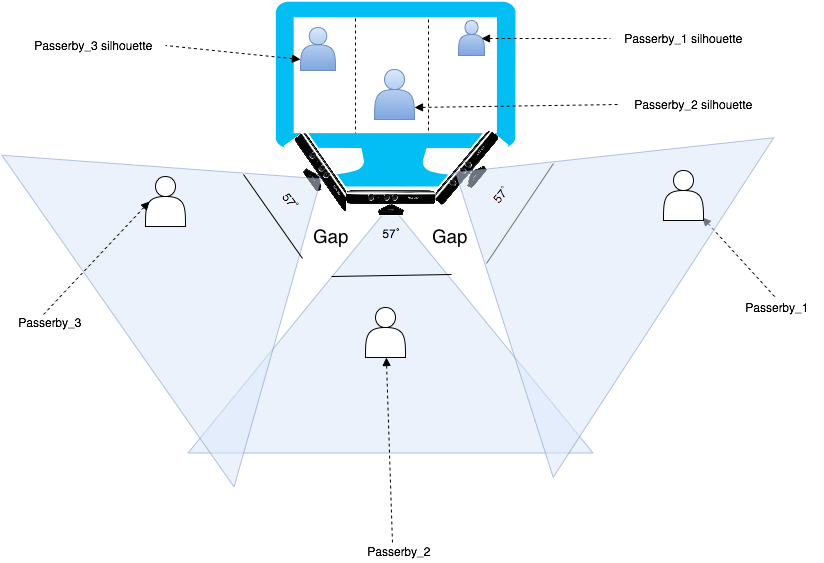
\includegraphics[width=0.9\textwidth,height=8cm]{Figures/9/Kinect_Extended}
    \caption{Attracting attention extended version.}%
    \label{fig:KinectExtended}%
\end{figure}


\section{Interaction design}
The interaction design for the extended version is completely the same as the body interaction design that was introduced in chapter 7. It consists of seven phases shown in figure \ref{fig:KinectExtended}.

\begin{enumerate}
\item \textbf{Passing by phase:} \\
This phase demonstrates passersby, who are not in the display tracking range.

\item \textbf{Implicit interaction phase:} \\
This phase starts, when passersby are in tracking range but are standing far or at side of the display. The range of this phase is extended in two sides shown in gray color.

\item \textbf{Subtle interaction phase:} \\
In this phase, the user is in near or center area of tracking range and facing toward display. The system motivates the user for direction interaction with the \emph{Call-to-Action} feature (``\emph{To play, Come near}'').

\item \textbf{Direct body interaction phase:} \\
This phase happens, when the user has actively started the game interaction and is playing. At this phase the whole tracking range (white color) could be used for direct interaction until the end of interaction phase.

\item \textbf{Watch ad video phase:} \\
When the interaction is over, a short advertisement video is shown.

\item \textbf{multi interaction phase:} \\
This phase demonstrates that the user can perform interaction multiple times.

\item \textbf{Follow up action phase:} \\
Follow up action phase is, when the user leaves the display’s tracking range and performs other actions.
\end{enumerate}


\begin{figure}[H]
    \centering
    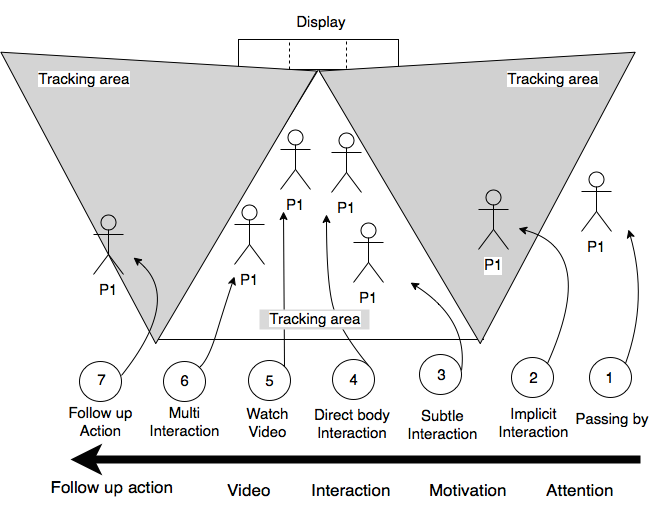
\includegraphics[width=0.85\textwidth,height=7.5cm]{Figures/9/enhanced_interaction_design}
    \caption{Extended Interaction design}%
    \label{fig:KinectExtended}%
\end{figure}




\section{Research question}
This experiment was conducted to find out that what are the major effects when the coverage area is expanded in both right and left side of the screen. This study compares the findings with the previous body interaction.

\begin{enumerate}
\item Would the attention level change?
\item Would the number of engaged passersby increase?
\item Would the average engagement time rise?
\item Would there be any changes in number of Honeypot and landing effect?
\item What would be the passersby behaviors to the display?
\end{enumerate}




\section{Study design}

\subsection{Location}
This experiment was conducted in the same location that was chosen for previous setup. It was positioned in the same pathway of passersby with the same height and screen brightness.  The surrounding of the display was also kept similar like the previous setup.

\subsection{Duration}
This experiment was conducted only for three continues days at end of the week, on Friday, Saturday and Sunday.

\subsection{Participants}
The participants were from Tourist information center. They were not informed that there was an interactive screen. Most of the participants were of old aged between 45-60, and the rest of participants were middle aged between 20-45 and. 

\subsection{Data gathering}
The below types of data were gathered during three days.

\begin{enumerate}
\item \textbf{On-Site Observation} \\
Two Observation slots were chosen, the first was from 10:00 – 12:00 and the second was from 14:00 – 16:00. During these two slots the below observations were made.

\begin{enumerate}
\item \textbf{Attention Level measurement} \\
Number of glances and number of ignores were counted by observing the passersby from a fixed location. Anyone who turned his/her face toward the display for less than 3 seconds were counted as \emph{Glanced}, and those who had not turned their faces at all were selected as \emph{Ignored}. See the full sheet of glances in Appendix \ref{app:EnhancedInteractiveadvertisementGlance}.

\item \textbf{Passerby behavior} \\
The behaviors of the passersby were observed by direct and indirect observations in onsite and from camera depth recordings. From the observations two important effects were taken in consideration, \emph{Honeypot} and \emph{Landing} effects. See other observation notes in Appendix \ref{app:EnhancedInteractiveobservationnotes}.



\end{enumerate}

\item \textbf{Depth recording} \\
A 2D colored image was recorded per second from each of three cameras simultaneously, which meanwhile were staked together side-by-side. At the end of day, another post processing script was applied to integrate a static background using Adobe Photoshop application. To match the data logs and the depth frames, each image name consisted timestamp as (12.43.21.png).
The below picture shows three Kinect images stacked together, as can be seen that people's colored images was rendered on the images (1,2 and 3). These images are stacked together so that the transition of one person be smooth from one camera to the other.


\begin{minipage}{0.95\textwidth}
\begin{flushright}
\begin{figure}[H]
   \centering
    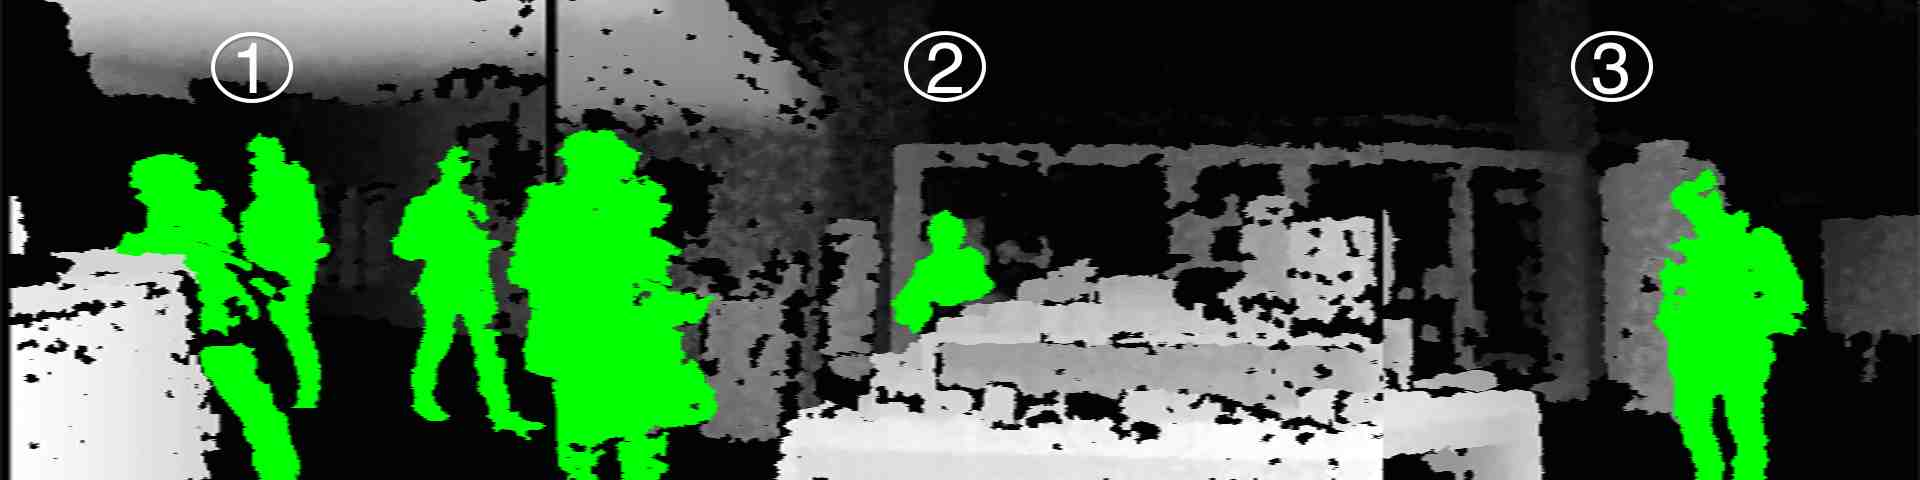
\includegraphics[width=\textwidth,height=40mm]{Figures/9/stacked_image}%
    \caption{Three Kinect images}%
    \label{fig:threekinectimages}%
\end{figure}
\end{flushright}
\end{minipage}


\end{enumerate}

\section{Findings and results}
This section first lists all the findings for enhanced version of advertisement, then it compares it with the previous interactive advertisement.


\subsection{Attention Level measurements}
The following chart shows the number of \emph{Glances} and \emph{Ignores} for the consecutive three days.

\begin{figure}[H]
    \centering
    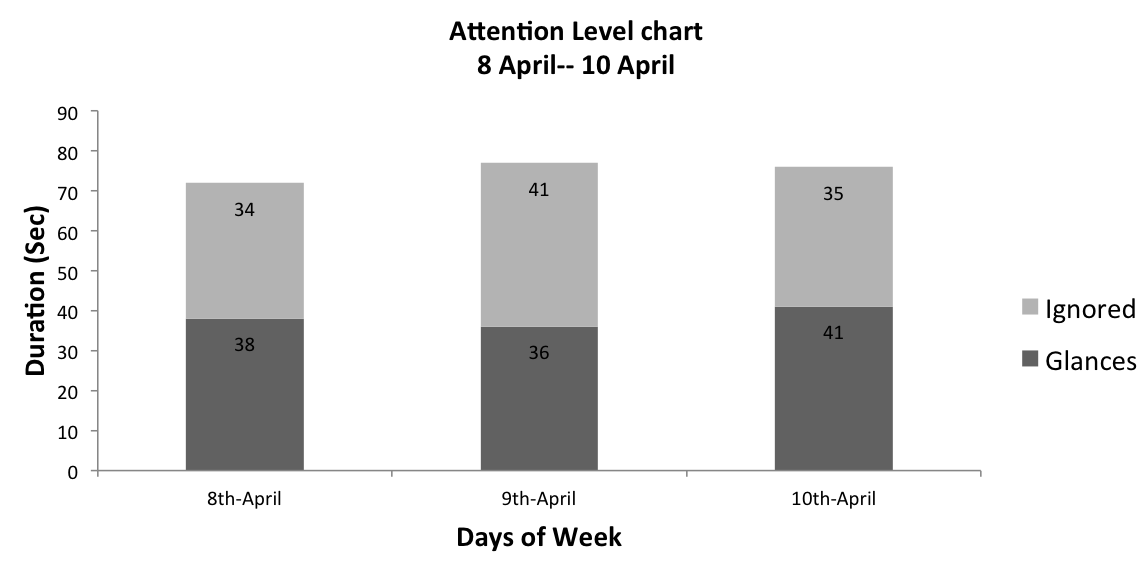
\includegraphics[width=110mm,height=55mm]{Figures/9/newbody_Inter_chart}%
    \caption{Attention level chart}%
    \label{fig:newbodyattentionlevelchart}%
\end{figure}


Each three days has almost similar number of \emph{Glances} and \emph{Ignores}. In average 51.11\% of passersby glanced and 49\% of passersby ignored the display.

\begin{figure}[H]
    \centering
    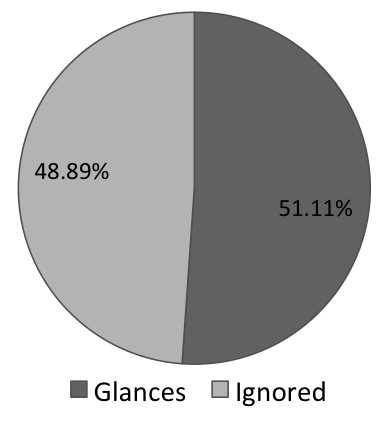
\includegraphics[width=60mm,height=55mm]{Figures/9/newbody_inter_percentage}
    \caption{Attention level percentage}%
    \label{fig:Nonattentionlevelpercentage}%
\end{figure}



\subsection{Times of Engagement phases}
The engagement time for each phase was counted from system logs and depth recording manually. The passersby spent 16.10 seconds in average for the first phase (\emph{Attraction/Motivation}), which had no specific duration to expire.  The same amount of average time (16.20 seconds) was spent for the \emph{Interaction phase}, which was restricted to only 40 seconds in max. And finally passersby spent only 3.63 seconds in average to watch advertisement video advertisement, which was limited up to 20 seconds.

\begin{figure}[H]
    \centering
    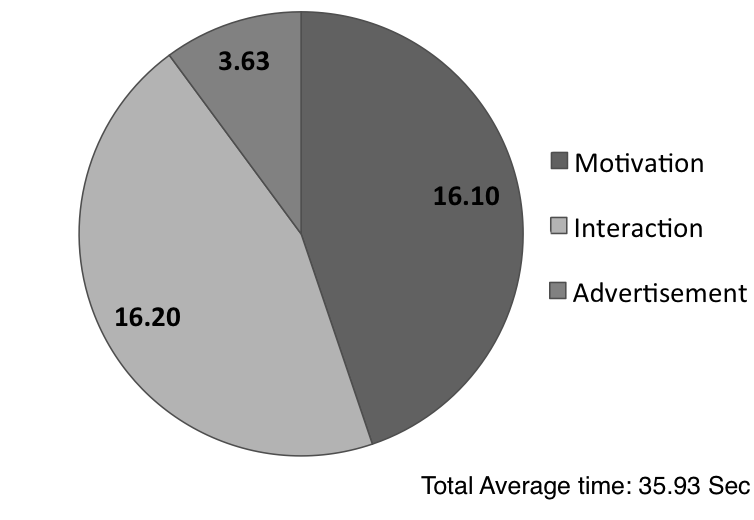
\includegraphics[width=90mm,height=60mm]{Figures/9/avg_phases}
    \caption{Average time for each phase}%
    \label{fig:newbodyaveragephases}%
\end{figure}

The entire average engagement duration for all these three phases together was around 36 seconds.


\subsection{Number of engaged passersby}
Each day’s depth recordings were watched and the numbers of passersby were counted manually. The people who stood in front of the screen for more than 3 seconds were flagged as \emph{Engaged} and the rest who ignored were flagged as \emph{Non-Engaged} passer-by. In total 104 passersby were engaged among 679 passersby with in three continues days. The below chart shows the \emph{Engaged} and \emph{Non-engaged} passersby for each single day.

\begin{figure}[H]
    \centering
    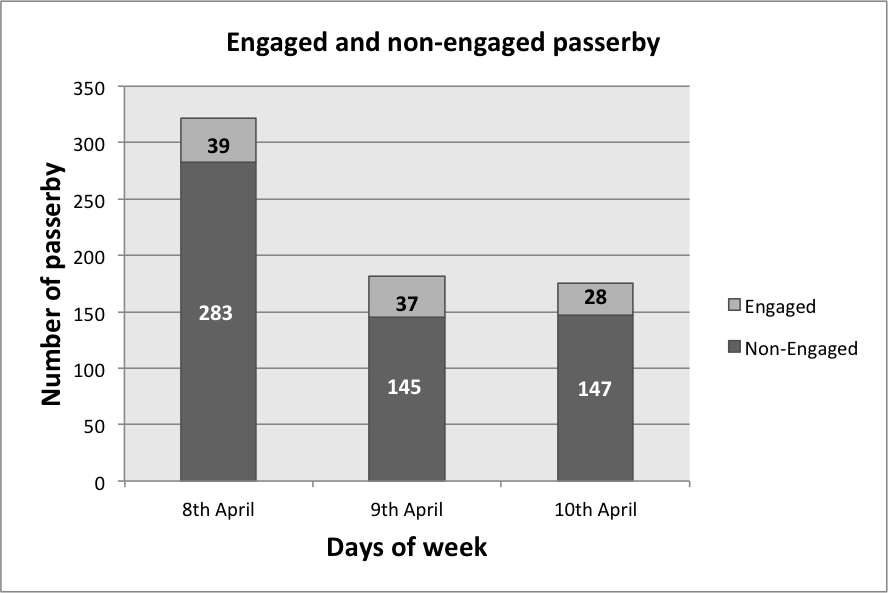
\includegraphics[width=0.9\textwidth,height=6.5cm]{Figures/9/newbody_inter_engage_day}
    \caption{Number of engaged passersby}%
    \label{fig:newbodyengagedandengagedby}%
\end{figure}


\begin{figure}[H]
    \centering
    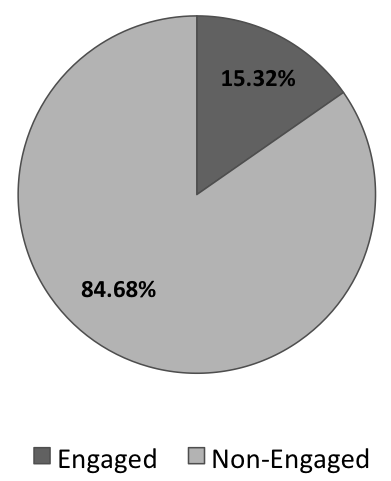
\includegraphics[width=60mm,height=60mm]{Figures/9/newbody_eng_percentage}
    \caption{Percentage of engaged and non-engaged passersby}%
    \label{fig:newbodyengagedpasserbypercentage}%
\end{figure}

The above pie chart is generated from all three days. It shows the percentage of passersby who were Engaged and not Engaged. In average 15.32\% of the whole population was \emph{Engaged} and 84.68\% were \emph{Non-Engaged}.


\subsection{Conversion funnel of engaged passersby}
To observe the depth of engagements, I used a \emph{Conversion-funnel} \cite{convfunnel} technique to illustrate how much passersby were engaged with this enhanced body interactive advertisement. The \emph{conversion-funnel} here presents the three layers of advertisement, \emph{Attention, interaction, ad video, and Action}. \emph{Action} is the ultimate goal of \emph{Bauhaus-Walk}, which is participation of passersby in the tour program. 

\begin{figure}[H]
    \centering
    \includegraphics[width=0.7\textwidth,height=7cm]{Figures/9/con-funnel}
    \caption{Conversion funnel of Engaged passersby}%
    \label{fig:bodyengagedpasserbypercentage}%
\end{figure}


As seen from the above chart, 104(100\%) passersby have been attracted and engaged to the advertisement, but not all passersby were interested to start the interaction. Only 61(58.6\%) passersby started the game interaction and had experienced with further advertisement elements. And among 61 participants, only 27(44\%) of them successfully completed the interaction and were exposed to the advertisement video, the rest of participants had left the interaction in the middle. The \emph{Action} (tour participation) was not counted because that could be influenced by many other existing advertisings from \emph{Bauhaus-Walk} in other locations.



\subsection{Landing and Honeypot effects}
Tow passersby behaviors were observed during the onsite and depth recording observations. These effects were \emph{Landing effect}\cite{LookingGlass} and \emph{Honeypot effects}\cite{EnticingPeople}. But these effects were not as strong as in previous body interaction technique. See the example frames below.



\begin{itemize}


\item Honeypot Effect:

\end{itemize}


\begin{wrapfigure}[22]{R}{0.55\textwidth}
  \vspace{-30pt}
  \begin{center}
    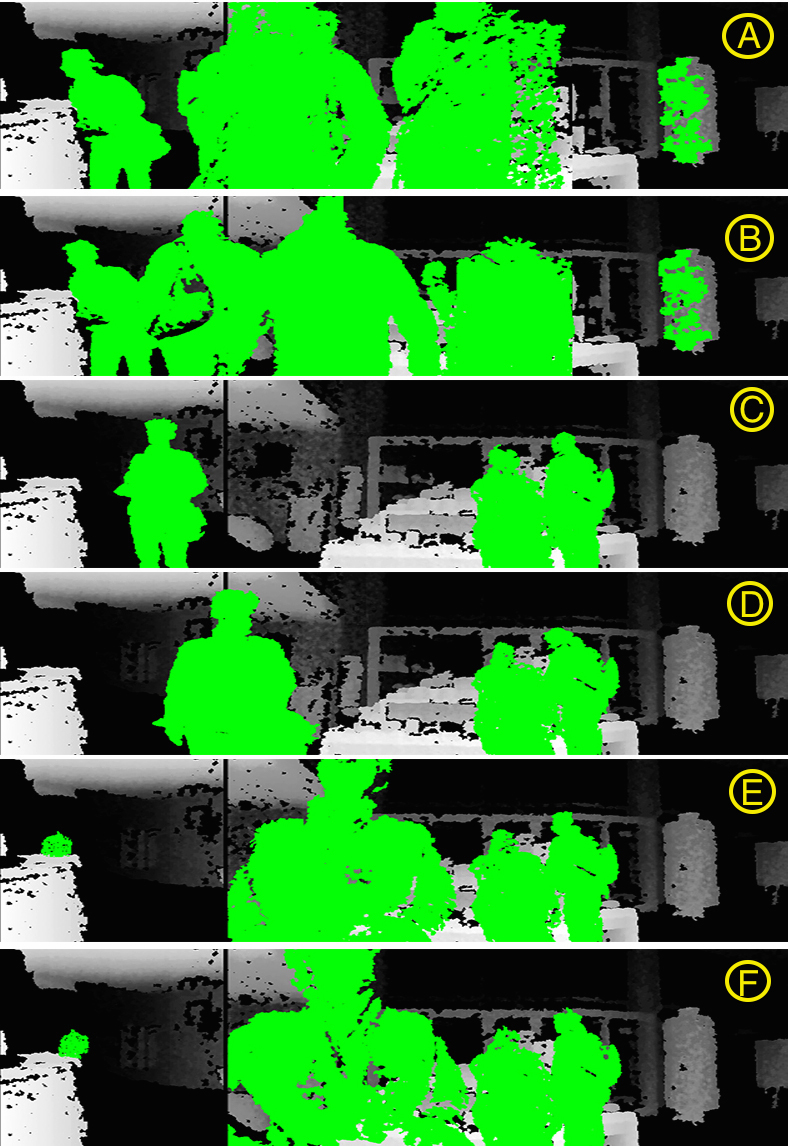
\includegraphics[width=0.55\textwidth,height=120mm]{Figures/9/effects/honeypot}
  \end{center}
  \vspace{-20pt}
  \caption{Honeypot effect}
  \vspace{-60pt}
\end{wrapfigure}
As can be seen from the picture in the right, which is composed of three kinect images that has covered right and left and the center of the display. 
In first frame (A) in the middle of the screen two persons are engaged and interacting for sometime. A women at the left is busy with the help desk, but she is curious about the screen and has got attracted toward the screen. She has looked many times toward the engaged people in previous frames. In frame (B) the two guys leave the interaction and walk away from the screen and the application is left alone. In frame (C) the women in the left is alone and is watching her self in the screen. She approaches toward the screen in frame (D). She is near to the screen and I guess realizes that the screen is in fact interactive and in frames (E, F) she comes closer and starts actively interaction.


 



%\begin{figure}[H]
%    \centering
%    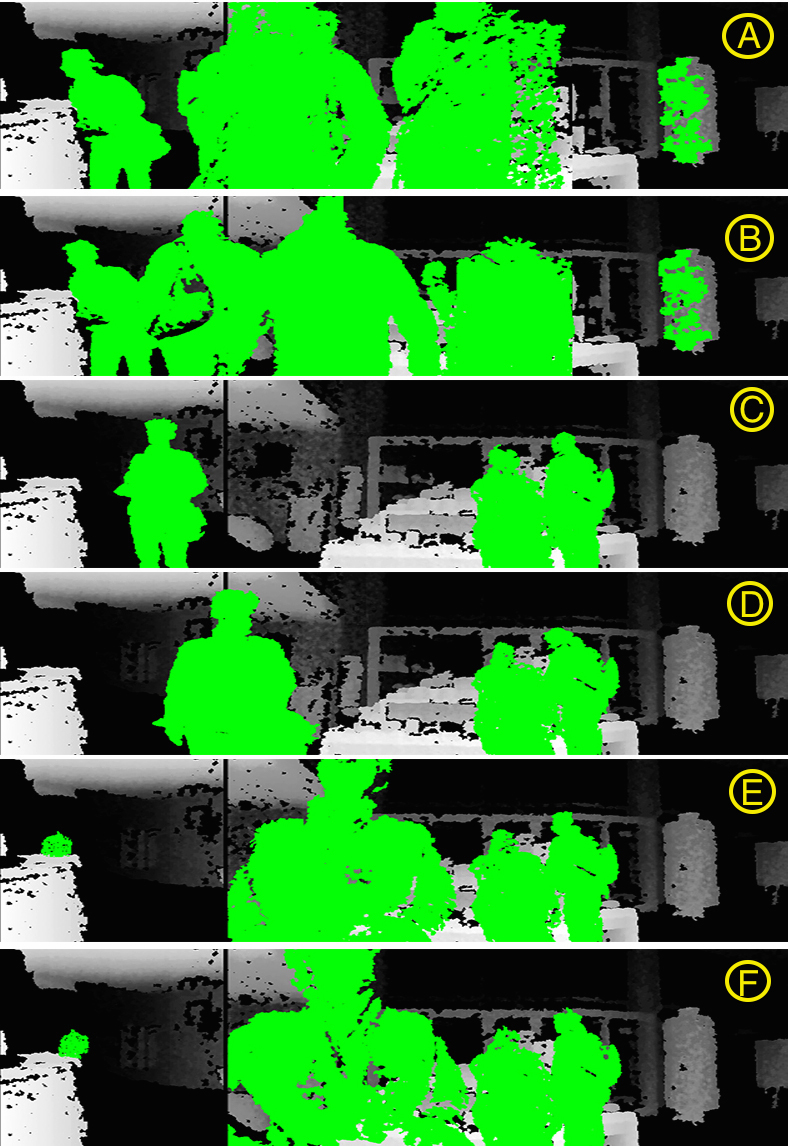
\includegraphics[width=0.6\textwidth,height=120mm]{Figures/9/effects/honeypot}
%    \caption{Honeypot effect}%
%    \label{fig:newbodyhoneypoteffect}%
%\end{figure}




\newpage
\begin{itemize}

\item Landing Effect:

\end{itemize}


\begin{wrapfigure}[30]{R}{0.55\textwidth}
  \vspace{-30pt}
  \begin{center}
    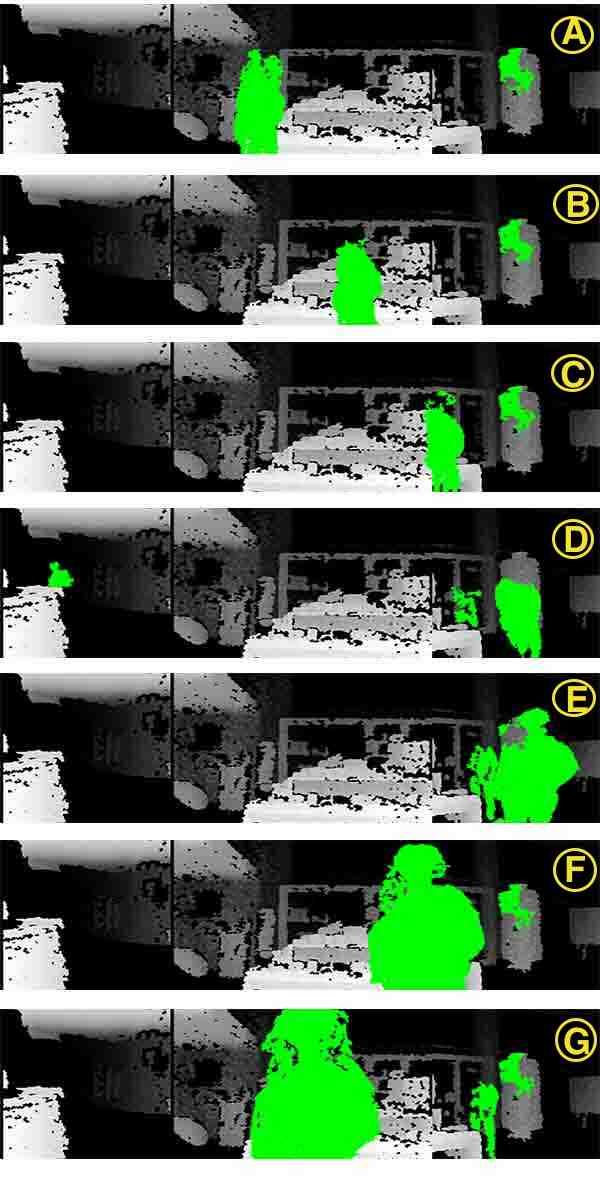
\includegraphics[width=0.55\textwidth,height=140mm]{Figures/9/effects/landing}
  \end{center}
  \vspace{-20pt}
  \caption{Landing effect}
  \vspace{-60pt}
\end{wrapfigure}
Few \emph{Landing effects} had also happened, which were similar to the previous experiments. The \emph{Landing effects} happened differently like, some noticed the interactivity in the middle and stopped by the display, and some noticed the interactivity at the very corner of the display and then moved back toward the screen.
As can be seen in the picture in the right, a lady is passing by the screen from frame (A – D) continuously without noticing anything. But she notices the screen interactivity at frame (E). She stops at her position for a second and when she realizes the interactivity then she moves closer to the screen in frame (F). She reaches the middle of the screen at frame (G) and starts to explore the game by interacting.
\break
\break
\break
\break
\break
\break
\break
\break
\break
\break
\break

The chart below shows the frequencies of \emph{Landing} and \emph{Honeypot} effects for three days. 



\begin{table}[H]
\centering
\label{tab:landingandhonypot}
\resizebox{7cm}{1.3cm}{
\begin{tabular}{| l | c | c |}
\toprule
\tabhead{Days} & \tabhead{Landing effect} & \tabhead{Honeypot effect} \\
\midrule
8th April   & 3   &  3 \\
9th April   & 2   &  5 \\
10th April  & 1   &  2 \\
\midrule
Total       & 6   &  10 \\
\bottomrule
\end{tabular}
}
\end{table}



\subsection{Other observations}
%see Appendix Appendix \ref{AppendixE}.2
Beside the above behaviors there were other observations recorded too as they are listed below. 
\begin{itemize}

\item Calling Others: \\
When a person is engaged with the display and is more excited about it, the person will most likely call his / her friend or family to see and give it a try. 
\end{itemize}

\begin{wrapfigure}[30]{R}{0.5\textwidth}
  \vspace{-10pt}
  \begin{center}
    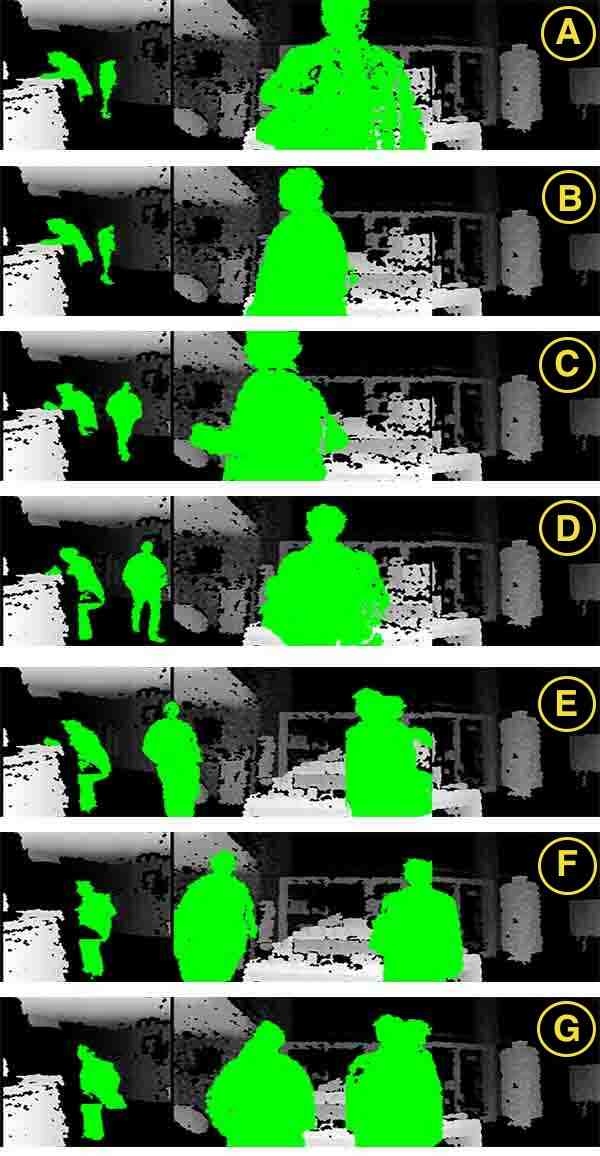
\includegraphics[width=0.50\textwidth,height=140mm]{Figures/9/effects/calling_others}
  \end{center}
  \vspace{-20pt}
  \caption{Calling others}
  \vspace{-20pt}
\end{wrapfigure}
Few of this \emph{Calling effects} have occurred in this enhanced version too, as can be seen in the picture in the right. A lady was engaged with the screen for a while in frame (A), she was standing in the middle of the screen. In frame (B) she turned herself and called her friend, who was standing very far from the display and was busy looking to some books. In frame (C) her friend left the work and started to look at her and moved toward the screen. In frame (D) the lady was back busy with the screen, when in frame (D) her friend came closer to the screen. In frame(F) she gave a bit space for her friend to let him see the screen. And finally her friend also started interacting and experiencing with the advertisement in frame (G).  
\break
\break
\break
\break
\break
\break
\break
\break
\break


\begin{itemize}
\item Noticing Interactivity earlier:
\end{itemize}


\begin{wrapfigure}[20]{L}{0.48\textwidth}
  \vspace{-30pt}
  \begin{center}
    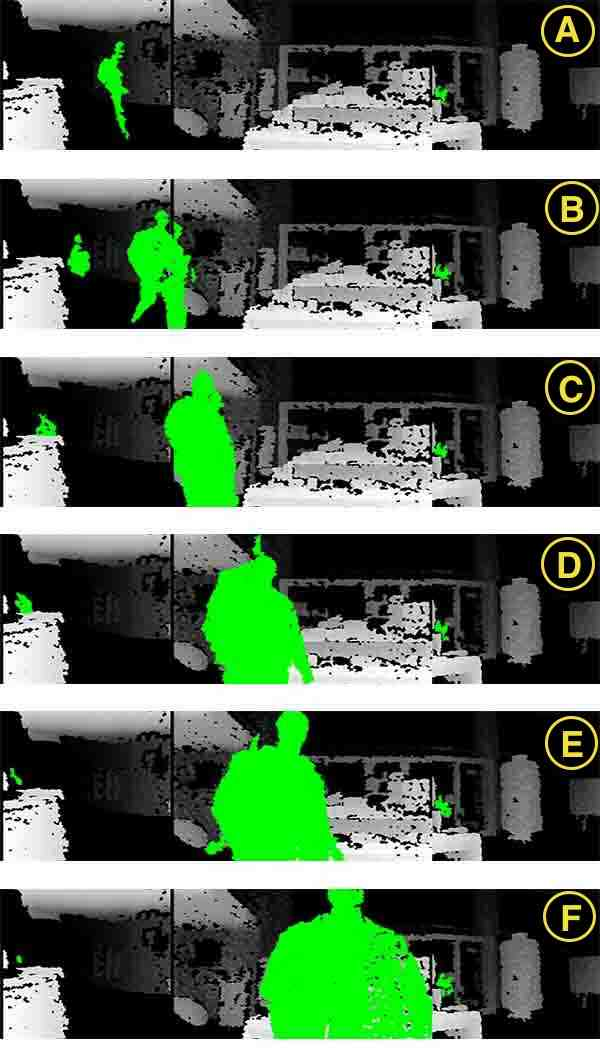
\includegraphics[width=0.45\textwidth,height=90mm]{Figures/9/effects/noticing_earlier}
  \end{center}
  \vspace{-20pt}
  \caption{Noticing interactivity earlier.}
  \vspace{-60pt}
\end{wrapfigure}
Passersby also directly came from the corners of display without any sign of\emph{Landing effect} toward the display and started interacting. This effect might have occurred because passersby had noticed themselves on the screen by the first camera, which was faced toward the side of the display. So it is assumed that they understood the interactivity and then came in the center of the display and started interacting. As can be seen from the image at the left side, a person was walking by from the left side in frame (A) and continued his walking toward the screen until the person got closer and closer toward the middle of the screen. It is obvious that he is not passing by the screen, but he intentionally stopped in the middle and started interacting. 
\break


\begin{itemize}

\item Side interaction:

\end{itemize}


\begin{wrapfigure}[25]{R}{0.48\textwidth}
  \vspace{-30pt}
  \begin{center}
    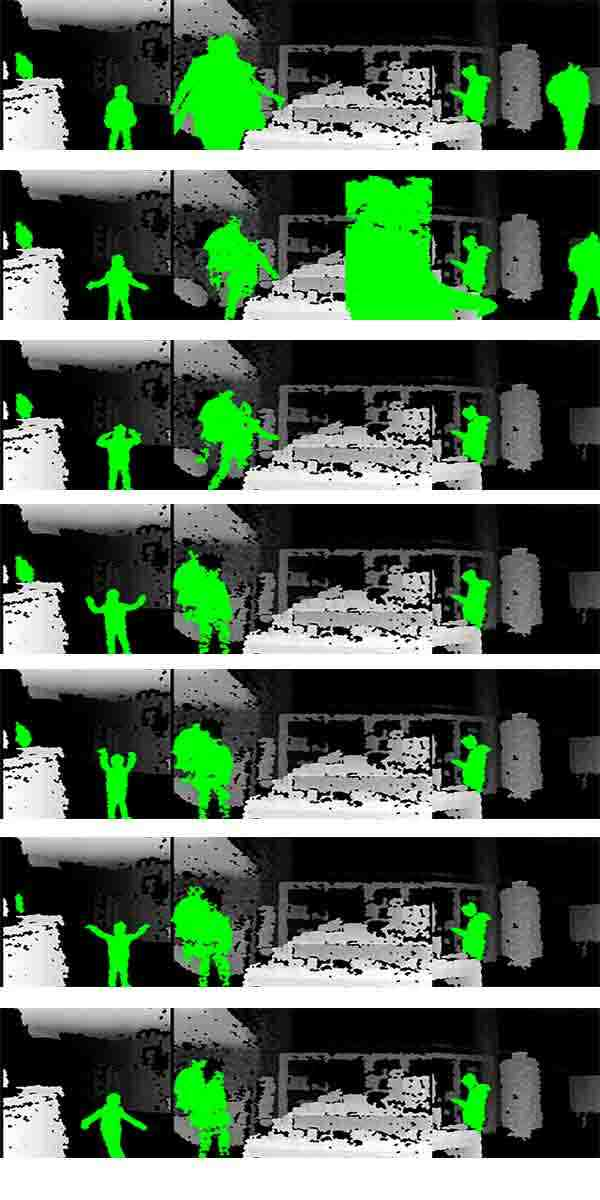
\includegraphics[width=0.48\textwidth,height=120mm]{Figures/9/effects/playing}
  \end{center}
  \vspace{-20pt}
  \caption{Side interaction}
  \vspace{-60pt}
\end{wrapfigure}
The integration of Kinect cameras at the side provided people with some sort of passive interactions. Passersby or people, who were standing at the side of the display and could not to come close to the screen, were still able to have some sort of connections with the system because they were tracked and shown. This feature provided a sense of safety comfort zone for them to stay back and still be able to interact passively. 

As can be seen in the picture in the right, there was a girl standing at the left side of the picture. She was standing with her parents at the information desk, and she recognized herself in the screen by waving her hand to confirm if it is actually her. And then she started to play with the silhouette on the screen and had fun for a while without coming closer.
\break
\break
\break
\break

\subsection{Comparison}
This section compares the results and findings of the enhanced version of advertisement with the previous advertisements, which could only track the middle screen of the display. 

\begin{enumerate}
\item \textbf{Comparison of number of passersby} \\
The number of passersby for different conditions may affect the findings. To be on safe side that the number of participants were statistically the same, the below computation has be applied on three similar days, which provides the base for further evaluations.


\begin{table}[H]
\caption{Number of people for three conditions}
\label{tab:newbodypasserbyofthreeweeks}
\centering
\resizebox{8cm}{1cm}{  
\begin{tabular}{| l | c | c | c |}
\toprule
\tabhead{Days} & \tabhead{Non-Interactive} & \tabhead{Body Interactive} & \tabhead{Enhanced body Interactive} \\
\midrule
\textbf{Day 1}  & 212 & 259 &  322 \\
\midrule
\textbf{Day 2}  & 209 & 216 &  182 \\
\midrule
\textbf{Day 3}  & 208 & 122 &  175 \\
\midrule
\textbf{Total}  & 629 & 597 &  679 \\
\bottomrule
\end{tabular}
}
\end{table}

\emph{ANOVA} test revealed that there was no statistical significant different between the passersby in each of the conditions (\emph{(F2,3)=0.1449, p >.05 (p=0.868)}). Because now the number of passersby were the same, I can perform other comparisons as below.


\item \textbf{Attention Level comparison}  \\
The number of \emph{Glances} and \emph{Ignores} for both body interactive, enhanced body interactive and non-interactive advertisements were collected as the following table lists.

\begin{table}[H]
\caption{Cross tabulation for each condition attention level}
\label{tab:newbodycrosstabulationweeks}
\centering
\resizebox{8cm}{1cm}{ 
\begin{tabular}{| l | c | c | c |}
\toprule
\tabhead{Method} & \tabhead{Glanced (\%)} & \tabhead{Ignored} & \tabhead{Total } \\
\midrule
\textbf{Non-interactive}     & 111(28.83\%)   &   274      &   385\\
\midrule
\textbf{Body Interactive}     & 106 (41.40\%)   &   150      &   256\\
\midrule
\textbf{Enhanced body Interactive }   & 115 (51.11\%)  &   110      &   225\\
\midrule
\textbf{Total }         		 & 332            &   534      &   866\\
\bottomrule
\end{tabular}
}
\end{table}


As can be seen the enhanced body interactive advertisement has a higher percentage about 51\% of the \emph{Glances} compared to the old body interactive advertisement. This means that there is a rise of 10\% increase. To test if these are statistically significant different, the \emph{Chi-Square} test was applied on them. The test revealed ${\chi}^2$\emph{(1, N=481)=4.5413, p < .05 (p=.033086)} they are statistically different and the enhanced body attraction technique does have a higher affect on the attention level. 

The non-interactive advertisement was about 28\% percentage in attracting attention, and the enhanced version had about 23\% higher attention level than non-interactive. The \emph{Chi-square} ${\chi}^2$\emph{(1, N=610)=30.2247, p < .001 (p=.0)}, strongly suggests that the enhanced version has dramatically increased the attention level than the non-interactive one.


\item \textbf{Engaged and Non-engaged passersby} \\
The numbers of \emph{Engaged} and \emph{Non-engaged} were recorded for all three conditions as below table demonstrates.

\begin{table}[H]
\caption{Number of engaged passersby in three weeks}
\label{tab:engagedofthreeweeks}
\centering
\resizebox{8cm}{1cm}{  
\begin{tabular}{| l | c | c | c |}
\toprule
\tabhead{Days} & \tabhead{Non-Interactive} & \tabhead{Body Interactive} & \tabhead{Enhanced body Interactive } \\
\midrule
\textbf{Day 1}  & 15 & 26 &  39 \\
\midrule
\textbf{Day 2}  & 15 & 20 &  37 \\
\midrule
\textbf{Day 3}  & 15 & 23 &  28 \\
\midrule
\textbf{Total}  & 45 & 69 &  104\\
\bottomrule
\end{tabular}
}
\end{table}


To find if the amount of \emph{Engaged} participants are different in these three conditions, \emph{ANOVA} test was applied. The test reveals that there was statistical difference between these conditions, (\emph{(F2,3)=20.3154, p <.05 (p=0.0021)}). But still it is unknown that which pairs were statistically different, therefore I run Post-Hoc Tukey’s HSD test as below.

\begin{table}[H]
\caption{Post-Hoc Tukey’s HSD}
\label{tab:engage-non-posthoctukey}
\centering
\resizebox{0.9\textwidth}{!}{  
\begin{tabular}{| l | c | c | c |}
\toprule
\tabhead{Methods} & \tabhead{Tukey HSD Q statistic} & \tabhead{Tukey HSD p-value} & \tabhead{Tukey HSD inferfence} \\
\midrule
\textbf{A vs B}  & 3.6459 & 0.0920761 &  insignificant  \\
\midrule
\textbf{A vs C}  & 8.9627 & 0.0017440 &  ** p<0.01 \\
\midrule
\textbf{B vs C}  & 5.3169 & 0.0218582 &  * p<0.05 \\

\bottomrule
\end{tabular}
}
\end{table}


Group A, B and C refers to Non-interactive, body interactive and enhanced body interactive advertisement subsequently. Post-hoc Tukey computed the critical value (Studentized Range Q statistic) for A and C as, ${Q}_{critical}^{\alpha=0.01,k=6}$ = 6.3250 and another critical value for B and C as, ${Q}_{critical}^{\alpha=0.05,k=6}$ = 4.3341. Based on the values, the significance can be determined if each pair’s critical value(Tukey HSD Q statistic) is bigger than Studentized Range Q statistic. ${Q}_{j}^{i }$ > ${Q}_{critical}$, and the strength of difference is determined by the \emph{P} value as shown above. 

From the diagram above it is very clear that non-interactive with body interactive is insignificant because their critical value is smaller than 4.3341 and p > 0.05. But the result was significant in the previous chapter because of all five days together but became insignificant with less number of days. On the other hand, the Non-interactive with enhanced body interactive is strongly significant because their critical value is bigger than 6.3250 with p < 0.01. The result of enhanced body compared to body interactive is also significant with p<0.05. As a result the enhance body interactive had strongly increased the number of \emph{Engaged} passersby compared to Non-interactive advertisement. The effect size between them are measured as below.

To find out how big was the difference between number of engaged passersby in non-interactive and enhanced body interactive conditions, the effect size by \emph{eta squared}(${\eta}^2$) was calculated. (${\eta}^2$) is an effect size index for \emph{ANOVA}, in which the $SS_{effect}$ (sum of squared) between conditions is divided by $SS_{total}$  (sum of squared) total. The below value was calculated by an online tool \emph{Easycalculator}\footnote{easycalculator: \url{https://www.easycalculation.com/statistics/eta-square-calculator.php}, last accessed 15 june 2016}.
\[
{\eta}^2 = \frac{{SS}_{effect}}{{SS}_{total}} = \frac{580.1687}{648.8354} = 0.8942\approx 0.89
\]

The 0.89 means that 89\% of total variance is accounted for by the conditions enhanced body interactive, non-interactive effects.




\item \textbf{Landing effect comparison}\\
The landing effects were recorded for non-interactive, body interactive and enhanced body interactive in below table.

\begin{table}[H]
\caption{Cross tabulation for each condition Landing effect }
\label{tab:newbodylandingeffect}
\centering
\resizebox{8cm}{1cm}{  
\begin{tabular}{| l | c | c | c |}
\toprule
\tabhead{Method} & \tabhead{Non-Interactive} & \tabhead{Body Interactive} & \tabhead{Enhanced body Interactive } \\
\midrule
\textbf{Day 1}    & 2    &   2      &   1\\
\midrule
\textbf{Day 2 }   & 0    &   2      &   2\\
\midrule
\textbf{Day 3}    & 1    &   3      &   3\\
\bottomrule
\end{tabular}
}
\end{table}
To find if the \emph{Landing effect} was different between these conditions. \emph{ANOVA} test applied, it states that there was no significant different between three days for all of the conditions, 
(\emph{(F2,3)=1.857, p >.05 (p=0.236)}).


\item \textbf{Honeypot effect comparison}\\
Honeypot effects were also gathered from those days as below in table.

\begin{table}[H]
\caption{Cross tabulation for each condition Honeypot effect }
\label{tab:newbodyhoneypoteffect}
\centering
\resizebox{8cm}{1cm}{  
\begin{tabular}{| l | c | c | c |}
\toprule
\tabhead{Days} & \tabhead{Non-Interactive} & \tabhead{Body Interactive} & \tabhead{Enhanced body Interactive } \\
\midrule
\textbf{Day 1}    & 2    &   2      &   3\\
\midrule
\textbf{Day 2 }   & 2    &   5      &   5\\
\midrule
\textbf{Day 3}    & 1    &   3      &   2\\
\bottomrule
\end{tabular}
}
\end{table}

ANOVA reveals that there is also no statistical difference between these three conditions too. 
(\emph{(F2,3)=1.667, p >.05 (p=0.266)})



\end{enumerate}

\section{Discussions}
The increase of attention level in enhanced body interactive advertisement version could have many reasons. (1)\emph{Wide angle tracking}, the wide angle of display tracking in which participants could see themselves from different sides (left, center and right), if they had missed the left there was still two chances to see the center or the other corner. (2) \emph{Exposure time}, the time passersby were exposed to their silhouette in three cameras facing (left, center, right) was longer than exposure time with only one camera. Normally it takes around 1.2 seconds to understand interactivity with silhouette with large screen that is in front of passersby \cite{ LookingGlass}.

\emph{Honeypot effect} in both body and enhanced body interaction evaluations did not seemed to be strong. There could be many general reasons for this effect, (1) \emph{Environment}, the display was situated in a touristic place, where people do not stay longer than staying in restaurant or some other gatherings. People move in and out often. (2) \emph{Unfamiliarity}, people are not familiar with each other to wait or come near to the shoulder of other person to look what is going on, as a result they tend to ignore display. (3) \emph{Personal interaction}, the interaction seemed more personal and single user,  and was not vast to be observed by others quickly. (4) \emph{Display size}, screen size was also small and passersby might have not noticed the interactions of people.

As mentioned before, \emph{Landing effect} happens, when the user notices interactivity after he passes by the screen. But in this enhanced version few \emph{Landing effects} happened. One of the reasons could be that when the passer-by was walking from a far side of the display, he was already noticing the interactivity because he could see himself in the screen. And when he reached near to the screen, he was aware of the interactivity for sure and would not perform landing. And by that time he would have two options (a) start interacting, or (b) ignore the interaction and pass by the screen.


\section{Conclusion}
In conclusion, the enhanced body interactive version performed significantly better than body interactive technique. It has increased the attention level of passersby and dramatically raised the number of \emph{Engaged} people in front of display. But the number of \emph{Landing} and \emph{Honeypot} effects were not significant compared to previous body interactive advertisement.

In enhance version, the number of \emph{Glances} were 51\% against the number of \emph{Ignore}. It was very effective in attention level than other two conditions (non-interactive and body interactive), because the number of \emph{Glances} were almost double than Non-interactive and 10\% increase than body interactive. The findings show that for a display positioned in a sideway, this technique can increase the attention level significantly than non-interactive display.

The enhanced version also increased the number of \emph{Engaged} people up to 15\% of whole passersby during three days, which the body interactive could not achieve in five days. The findings state that the enhanced version significantly engaged people than body interactive, but the significance was not as strong as compared to Non-interactive which was above the double of percentage of engaged. 

The above percentages could have increased if the silhouette color was not the same for all passersby. Representation of different silhouette colors can have effect on the attention level, and it might motivate passersby to get closer and get engaged. it would be very effective if this concern gets improved in future.





